\documentclass{beamer}
\DeclareFontShape{OT1}{cmss}{b}{n}{<->ssub * cmss/bx/n}{} 
\usetheme{default}
\usepackage{amsmath}
\usepackage{amsfonts}
\usepackage{mathbbol}
\usepackage{xcolor} % before tikz or tkz-euclide if necessary
\usepackage{tkz-euclide} % no need to load TikZ
\usepackage{multirow}
\usepackage{lmodern}
\usepackage{bm}

\title{Statistical Machine Learning\\ Part 7\\
Tree-Based Methods}
\author{Horacio G\'omez-Acevedo\\ Department of Biomedical Informatics\\
University of Arkansas for Medical Sciences}
\begin{document}
	\begin{frame}[plain]
		\maketitle
	\end{frame}
	
	
	\begin{frame}{Tree structures}
		
		A typical tree is depicted with the root being the top node, and growing down. Decisions are being made at each node until a terminal node or {\it leaf} is reached. Each non-terminal node contains a question on which a split is based. Each leaf contains the label (classification) or the predicted mean value (regression).
		 
		
		
\end{frame}

\begin{frame}{Regression Trees}

We will use the {\bf Hitters} data set as an example for  regression.  After running the code we obtain the following figure

\begin{figure}[h]
	\centering
	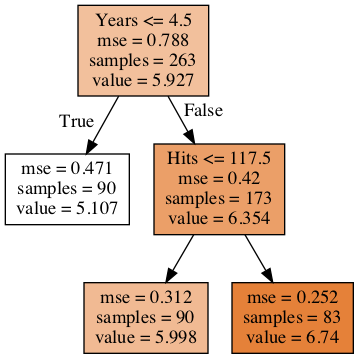
\includegraphics[scale=0.5]{../../Figures/fig_hitters.png}
\end{figure}
	
	
\end{frame}

\begin{frame}{Regression Trees (cont)}
	How to read this information?
	The main feature for this set is {\it years}, from which the total samples are split into two depending on whether their time spent in the baseball league has been less than 4.5 years. The case on the left (True) is already given a value of $5.107$, which means that the average salary is $\exp(5.107)\approx 165.17$ thousand dollars a year. Players with more than 4.5 years will be further divided into the variable ${\it hits} $, and someone above 117.5 will earn on average $\exp(6.74)=845.56$ thousand dollars!
\end{frame}

\begin{frame}{Regression Trees (cont)}
	We can see that the graphical representation of a tree is as follows
	
	\begin{figure}[h]
		\centering
		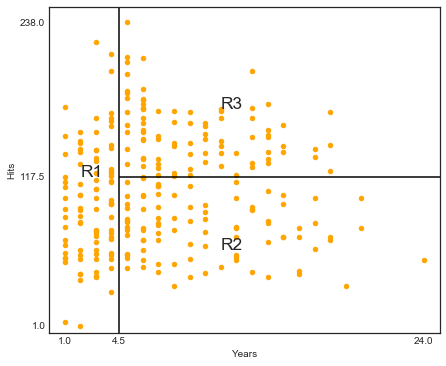
\includegraphics[scale=0.5]{../../Figures/fig_hitters_graph.png}
	\end{figure}
The regions $R_i$ are the representing the leaves of the tree.  	
	
\end{frame}

\begin{frame}{Prediction in Regression Trees}
	There are two main steps involved in building a tree
	
	\begin{itemize}
		\item Divide the predictor space $X_1 \times X_2 \times \cdots \times X_p$ into $J$ distinct and non-overlapping regions $R_1,\ldots, R_J$.
		\item For every observation that falls into the region $R_j$, we make the same prediction, which is the mean of the response values for the training observations in $R_j$.
	\end{itemize}
\end{frame}

\begin{frame}{2D Example}
	Suppose we have the outcome $Z$ depending on two predictors $X$ and $Y$ defined in certain rectangular area $A\subset X \times Y$ of the plane. One feasible partition of $A$ is depicted below
		\begin{figure}[h]
		\centering
		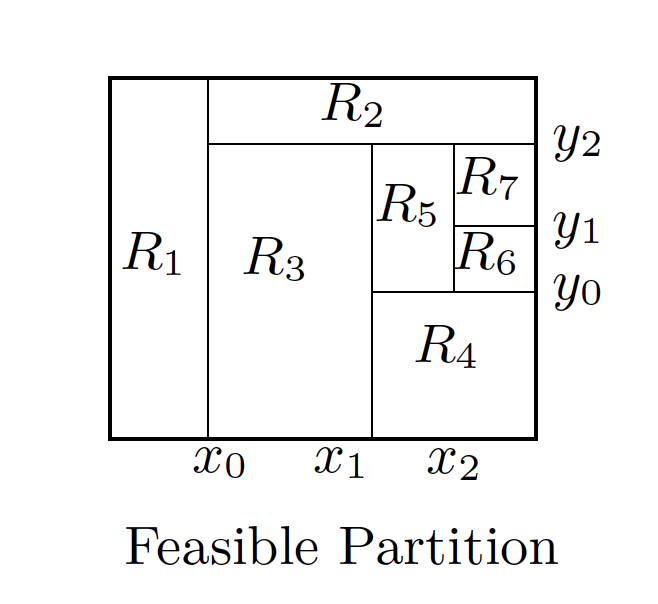
\includegraphics[scale=0.5]{../../Figures/fig_tree_region.png}
	\end{figure}
	
\end{frame}

\begin{frame}{2D Example (cont)}
The previous partition can be described as a tree structure
\begin{figure}[h]
	\centering
	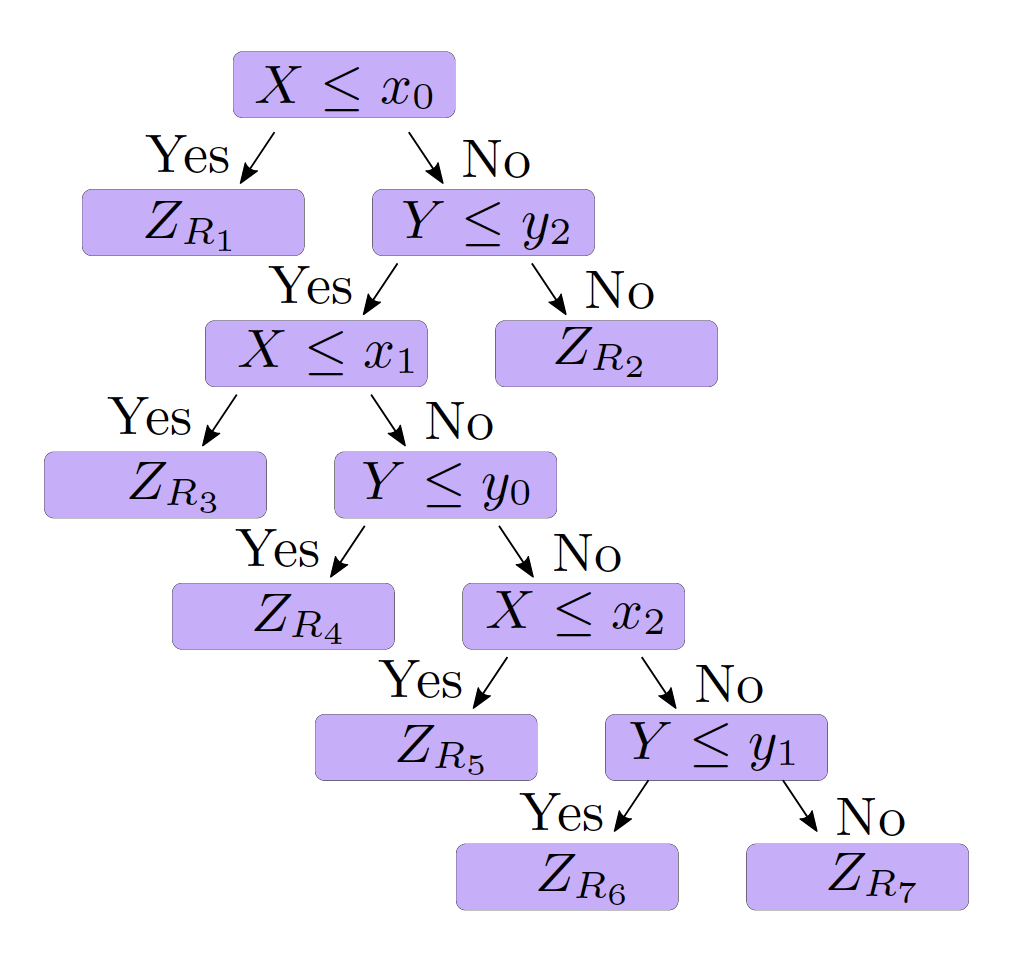
\includegraphics[scale=0.3]{../../Figures/fig_tree_trans.png}
\end{figure}

The corresponding prediction for $\widehat{Z}(x,y)$ based on given partition of $A$ is defined as 
\begin{equation*}
	\widehat{Z}(x,y)= \textrm{Average} \{ Z(x_r,y_r)\colon (x_r ,y_r)\in R_j)\}
\end{equation*}
where $(x,y) \in R_j$.

\end{frame}

\begin{frame}{Dividing the Predictor Space}
	Ideally, one must find regions $R_1, \ldots, R_J$ (also called {\bf boxes}) that minimize the $RSS$ given by 
	\begin{equation*}
		\sum_{j=1}^J \sum_{i\in R_j} (y_i - \hat{y}_{R_j})^2
	\end{equation*}
where $\hat{y}_{R_j}$ is the mean response for the training observations within the $j$th box. Since it is not computationally feasible to test every single box combination, we use a {\it greedy} approach that is known as {\it recursive binary splitting}. This process is top down since we start with the whole reagion and after a number of successive splits into two branches further down on the tree. At each step we select the {\it best} split at the given time without looking at other alternatives further down. 
\end{frame}

\begin{frame}{Recursive Binary Splitting}
	We begin by selecting a predictor $X_j$ and the cutpoint $s$ sucha that splitting the predictor space into the regions $\{ X| X_j <s \}$ and $\{ X | X_j \ge s\}$ leads to the greates possible reduction in RSS. Thus, for any $j$ and $s$, we define a pair of half-planes
	\begin{equation*}
		R_1(j,s)= \{ X | X_j <s\} \quad \textrm{and } R_2(j,s)= \{X| X_j\ge s\}
	\end{equation*}
and we look for the value $j$ and $s$ that minimize the equation
\begin{equation}
	\sum_{i: x_i \in R_1(j,s)} (y_i - \hat{y}_{R_1})^2 + 	\sum_{i: x_i \in R_2(j,s)} (y_i - \hat{y}_{R_2})^2 ,
\end{equation}
We repeat the process looking for the best predictor and best cutpoint in order to split the data further so as to minimize the RSS within each of the resulting regions but this time we we don't split the entire space but each of the two regions found. This process continues until a certain criteria is reach (e.g., until no region contains fewer than a certain number of elements within). 


\end{frame}

\begin{frame}{Recursive Binary Splitting (cont)}

Once the regions are found, the predicted response for a given test observation is the mean of the training observations in the region to which that test observation belongs.

The recursive binary splitting may produce good predictions on the training set, but it follows to close the data and more likely produce overfit. Thus, a smaller tree with fewer splits might lead to lower variance and better interpretation at the cost of bias.
\end{frame}

\begin{frame}{Tree Pruning}
	
	
	One way to address the overfiting problem is to grow a very large tree $T_0$ , and then prune it back to obtain a sub-tree. Ideally, we select a sub-tree that leads to the lowest test error rate using say cross-validation. 
	
	Once again we faced the  problem that the number of possible sub-trees is computationally intensive.
	
	A process known as {\it weakest link pruning} considers a sequence of trees indexed by a non-negative tuning parameter $\alpha$. For each value of $\alpha$ there corresponds a sub-tree $T \subset T_0$ such that the following quantity is as small as possible
	
	\begin{equation}
		\sum_{m=1}^{|T|} \sum_{i\in R_m} (y_i -\hat{y}_{R_m})^2 + \alpha |T|,
	\end{equation}
	 where $|T|$ denotes the number of leaves of the tree $T$.
\end{frame}


\begin{frame}{Regression Tree Algorithm}
	\begin{enumerate}
		\item Use recursive binary splitting to grow a large tree on the training data. Use a stopping rule such as the minimum number of observations on each leaf.
		\item Apply the weakest link pruning  to the large tree in order to obtain a sequence of best sub-trees as a function of a parameter $\alpha$. 
		\item Use $K$-fold cross-validation to choose $\alpha$. More precisely, divide the training observations into $K$ folds, and for $k \in \{1,\ldots, K\}$ do:
		\begin{enumerate}
			\item Repeat steps 1 and 2 on all but the $k$th fold of the training data.
			\item Evaluate the mean squared prediction error on the data in the left-out $k$th fold, as a function of $\alpha$
		\end{enumerate} 
		Average the results for each value of $\alpha$, and pick $\alpha$ that minimize the average error.
		\item Return the sub-tree from step 2 that corresponds to the chosen value of $\alpha$.
	
	\end{enumerate}
\end{frame}

\begin{frame}{Example. }
	The unpruned tree that results from greedy splitting on the training data from the {\bf Hitters} dataset is depicted below

\begin{figure}[h]
	\centering
	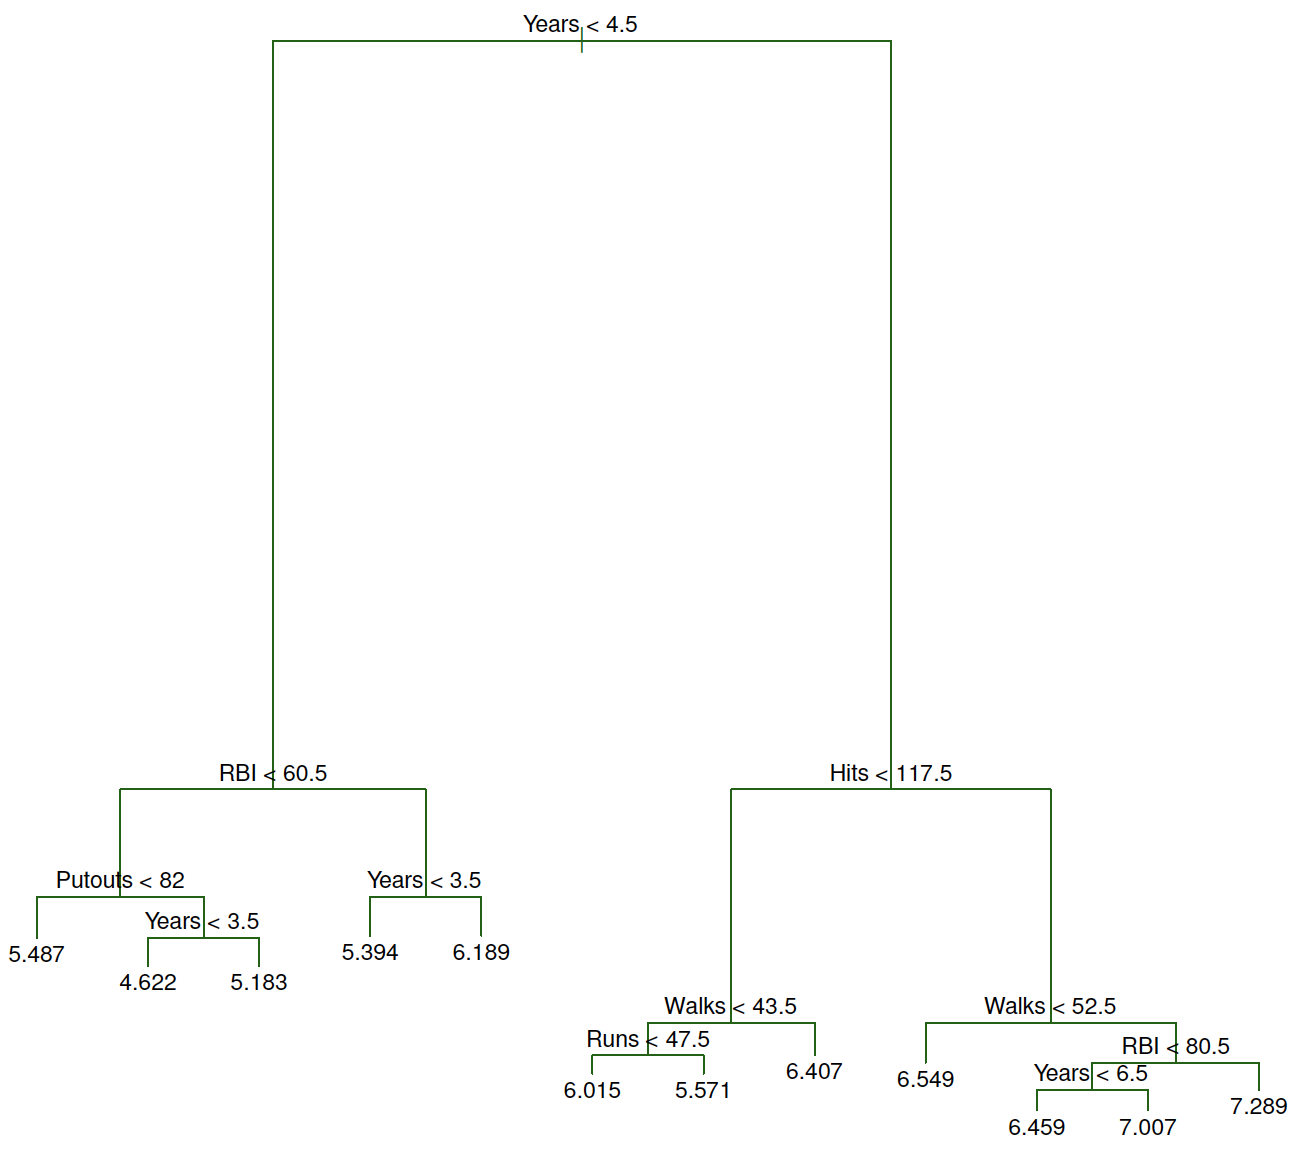
\includegraphics[scale=0.3]{../../Figures/fig_hitters_full.png}
\end{figure}
\end{frame}

\begin{frame}{Example (cont)}
	\begin{figure}[h]
		\centering
		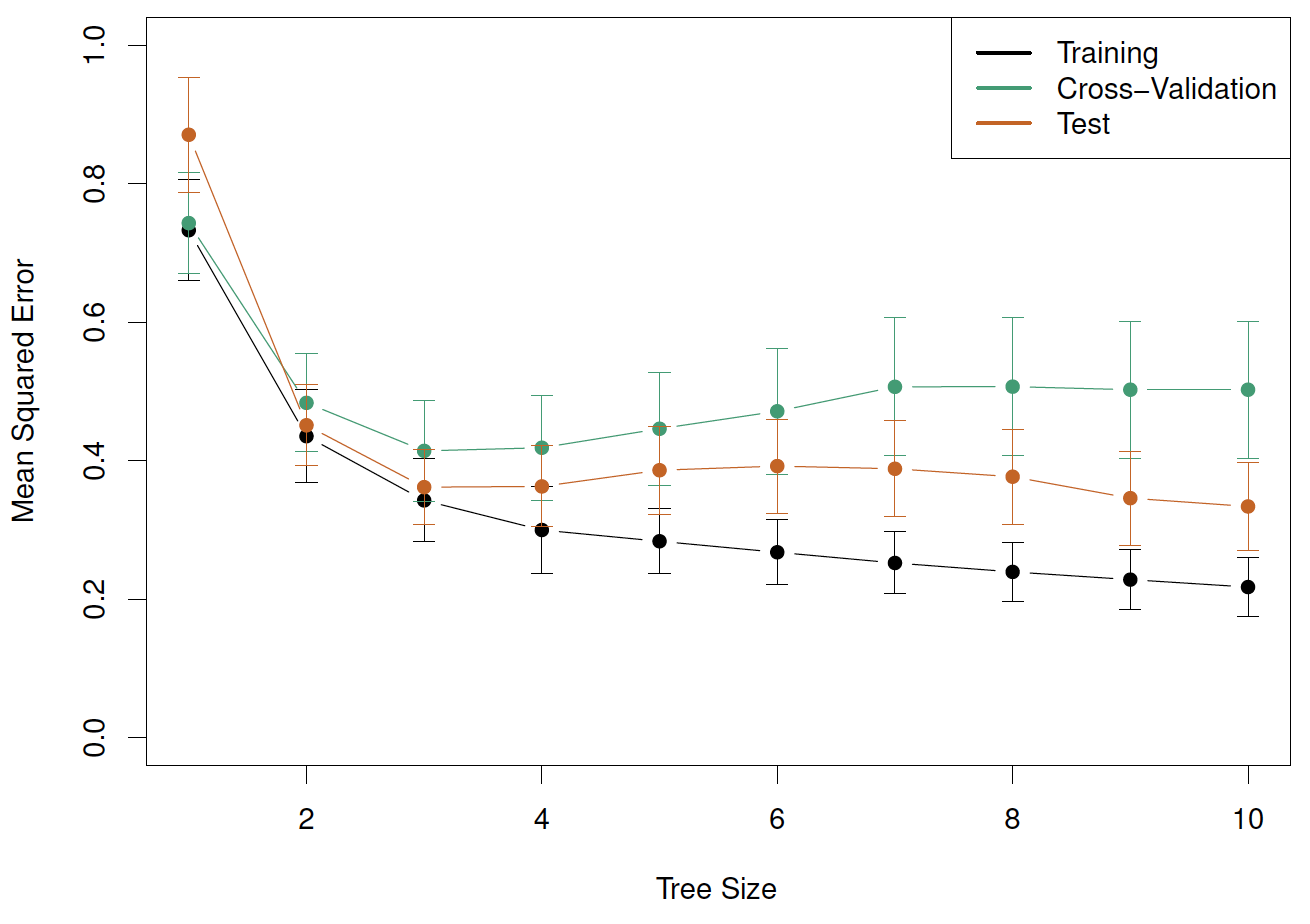
\includegraphics[scale=0.4]{../../Figures/fig_hitters_mse.png}
	\end{figure}
\end{frame}

\begin{frame}{Classification Trees}
	The idea of the classification trees is very similar to the regression trees. However, in the classification setting we cannot use RSS as an splitting criteria for the binary selection. Instead, we will use the {\bf classification  error rate}, which is the fraction of the training observations in a region that do not belong to the most common class.
	\begin{equation*}
		E= 1- \max_k (\hat{p}_{mk})
	\end{equation*} 
	where $\hat{p}_{mk}$ represent the proportion of training observations in the $mt$h region that are from the $k$th class.	
	

\end{frame}

\begin{frame}{Purity metrics}
	
	A node is {\bf pure} if all training instances belong to the same class. 
	Some metrics to asses the impurity are:
	\begin{itemize}
		\item {\bf Gini index.} Defined by
		
		\begin{equation*}
			G= \sum_{i=1}^K \hat{p}_{mk} (1 - \hat{p}_{mk}),
		\end{equation*}
		is a measure of total variance across the $K$ classes. 
	\item {\bf Cross-entropy. } Defined by
	\begin{equation*}
		D = - \sum_{k=1}^K \hat{p}_{mk}\log \hat{p}_{mk}.
	\end{equation*}	
	Note that both metrics will take on a small value if the $m$th node is pure. Both the Gini index and the cross-entropy are quite similar numerically. 
\end{itemize}
	
\end{frame}

\begin{frame}{Example}
	
	Using the {\bf Heart} data, the classification tree (unpruned) is shown below. 
	\begin{figure}[h]
	\centering
	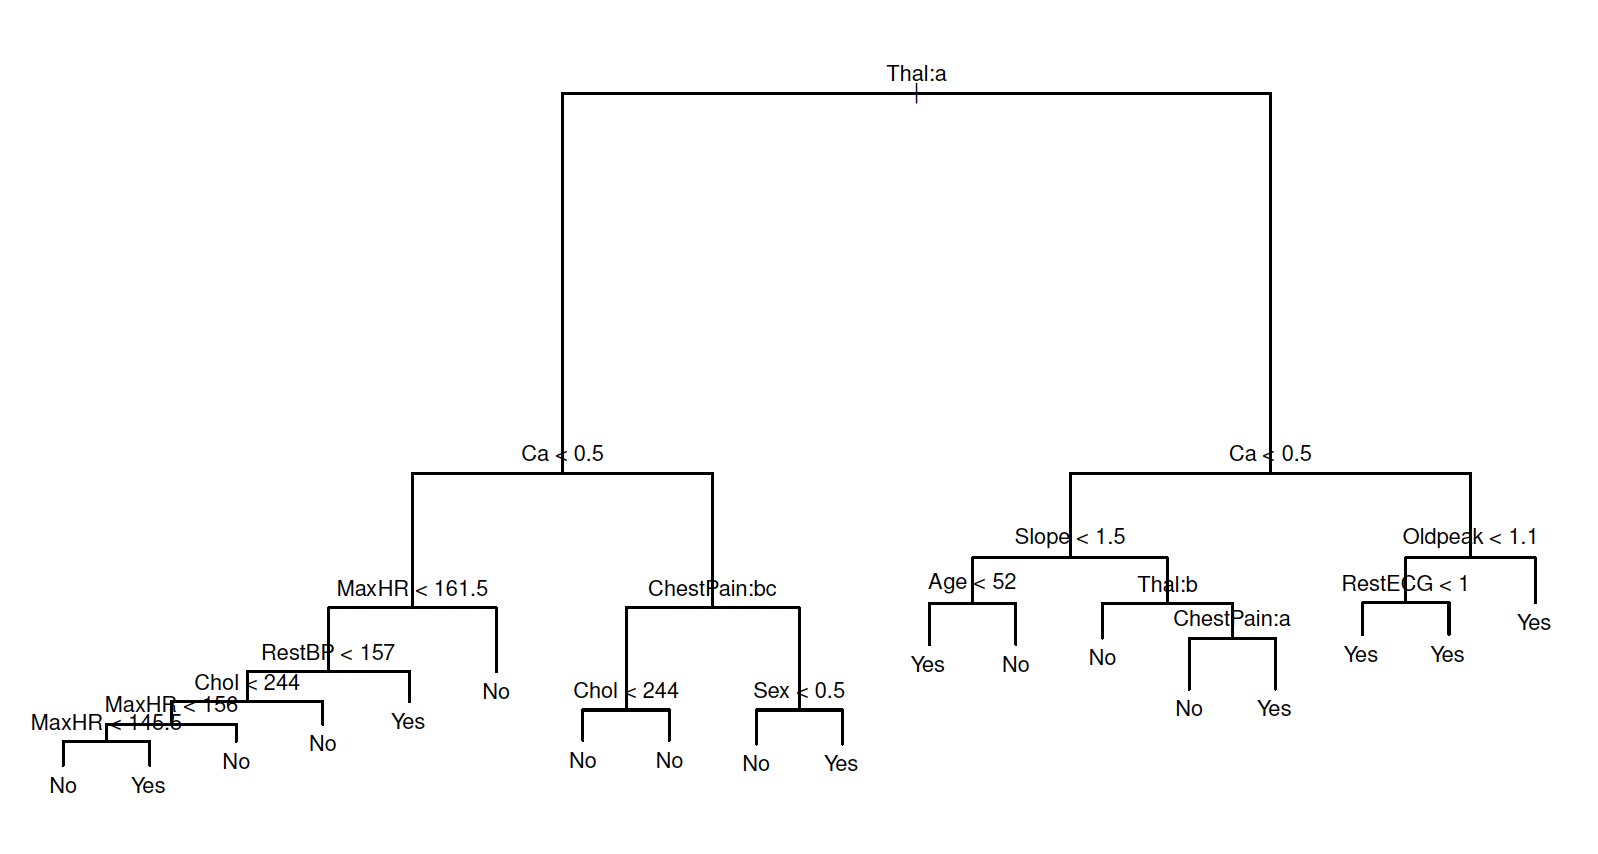
\includegraphics[scale=0.3]{../../Figures/fig_class_tree.png}
\end{figure}	
Note the leave {\tt RestECG<1} . The response is Yes so why do we need to partition further? Then answer is that it does not reduce the classification error but  it improves the Gini index and cross-entropy. 
\end{frame}
	
\begin{frame}{Example (cont)}
	Cross-validation error, training and test error 
	
		\begin{figure}[h]
		\centering
		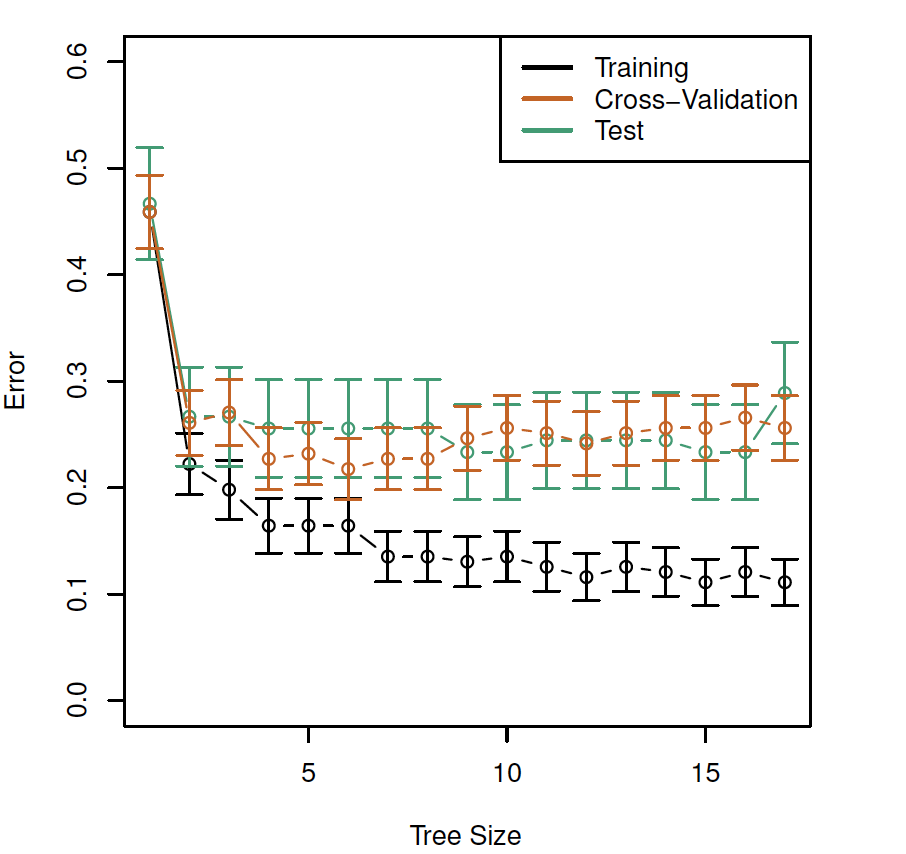
\includegraphics[scale=0.4]{../../Figures/fig_class_tree_error.png}
	\end{figure}
	
\end{frame}

\begin{frame}{Trees vs. Linear Models}
	The classical linear regression assumes a relationship of the form
	\begin{equation*}
		f(X)= \theta_0 + \sum_{i=1}^p \theta_j X_j
	\end{equation*}
whereas the regression trees assume that the model has the form
\begin{equation*}
	f(X)=\sum_{i=1}^M c_m \cdot 1_{X \in R_m}
\end{equation*}
where $R_1,\ldots,R_M$ represent a partition of feature space and $1_A$ represents the indicator function (1 if $x\in A$ and 0 elsewhere)
\end{frame}

\begin{frame}{References}

Materials and some of the pictures are from (1),(2), and (3).
\begin{enumerate}
	\item Gareth James et al. {\it An Introduction to Statistical Learning with applications in R}. Springer (2015)
	\item Brian D. Ripley {\it Pattern Recognition and Neural Networks}. Cambridge University Press (1996). 
	\item Aur\'elien G\'eron. {\it Hands-on Machine Learning with Scikit-Learn \& TensorFlow} O'Relly (2017)
	\item Wiebe R. Pestman {\it Mathematical Statistics} de Gruyter (1998)
	
\end{enumerate}	

I have used some of the graphs by hacking TiKz code from StakExchange, Inkscape for more aesthetic plots and other old tricks of \TeX
\end{frame}	


\end{document}
